\chapter{Continuo tridimensionale}


\section{Introduzione}
Essendo ormai diventati familiari con la descrizione  della cinematica del continuo, intenzionalmente limitata finora al contesto monodimensionale, il passaggio al quadro concettuale della formulazione tridimensionale più realistica dovrebbe essere naturale e quasi evidente. Alcuni aspetti tecnici coinvolti, tuttavia, sono più che semplici generalizzazioni. In una dimensione spaziale, ad esempio, la nozione di rotazione è completamente assente e, pertanto, la formulazione tridimensionale deve affrontare il problema di come escludere le rotazioni del corpo rigido dal processo di deformazione. Un'altra differenza essenziale è data dal fatto che la frontiera di un dominio monodimensionale consiste in una collezione disgiunta (di due punti di confine), mentre in due o più dimensioni spaziali la frontiera è essa stessa un dominio continuo, un fatto che ha ripercussioni sulla formulazione dei problemi  e sui metodi di soluzione delle equazioni differenziali alle derivati parziali che li governano.


\section{Deformazione}

Continueremo ad identificare un \textit{corpo}  $\Bc$ è una varietà di \textit{punti materiali}, che denotiamo con $X$ e supporremo che sia  in grado di occupare varie  regioni dello spazio ambiente, che adesso identifichiamo con lo spazio Euclideo tridimensionale $\Ec$. Indicheremo con $\Vc$ l'associato spazio vettoriale delle traslazioni.

Osserviamo i corpi sullo sfondo di questa struttura spaziale,  uno sfondo che svolge il ruolo del muro osservato dai prigionieri nella caverna di Platone. A differenza di quei prigionieri, non siamo interessati a rompere le nostre catene e correre fuori per ottenere esperienza del mondo ``reale'' esterno, solo per tornare nella caverna e confrontare le ombre sul muro con i loro ``veri'' corrispondenti. Semplicemente non ci consideriamo prigionieri e ci  preoccupiamo piuttosto di fornire un modello matematico del nostro unico dato d'esperienza, quelle ombre.

Come prima, la varietà $\Bc$ è generalmente assunta regolare, ovvero un diffeormorfismo di un dominio nello spazio Euclideo. In particolare, affermiamo che un insieme aperto $\Omega$ nello spazio $\Ec$ è occupato dal corpo $\Bc$ qualora esista una funzione \textit{iniettiva}, denominata \textit{piazzamento} o \textit{configurazione}, che mappa $\Bc$ in $\Omega$:
\begin{equation}
	\kappa\,:\,\Bc\to \Omega\in \Ec.
\end{equation}
Il piazzamento $\kappa$ mappa dunque i punti materiali $X$ in elementi $\xb$ dello spazio $\Vc$ tridimensionale; $\xb$ è dunque la posizione occupata dal punto $X$ nel piazzamento $\kappa$. In maniera un po' imprecisa chiameremo $\xb$ un ``punto'', intendendo per tale la posizione occupata da $\kappa(X)$. Analogamente scriveremo $\xb\in \Omega$, immaginando di identificare $\Omega=f(\Bc)$ con l'insieme delle posizioni dei suoi punti.

\begin{figure}
	\centering
	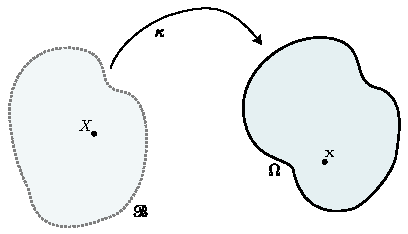
\includegraphics[scale=1.2]{figure/cinematica/piazzamento3d}
	\caption{Piazzamento $\kappa$.}
	\label{fig:piazzamento3d}
\end{figure}

Se $\chi$ è un altro piazzamento, possiamo definire la funzione
\begin{equation}
	\fb\,:\, \kappa(\Bc)\mapsto\chi(\Bc)
\end{equation}
come $\fb\coloneqq\chi\circ \kappa^{-1}$. Tale funzione è la \textit{deformazione} dalla configurazione $\kappa$ alla configurazione $\chi$. A differenza di quanto accadeva nel caso monodimensionale, osserviamo che adesso $\fb$ è un campo vettoriale. Dunque, se $\xb=\kappa(X)$, diremo che $\xb$ e $\fb(\xb)$ sono rispettivamente le posizioni occupate dal punto materiale $X$ prima e dopo la deformazione $\fb$.

\begin{figure}[h]
	\centering
	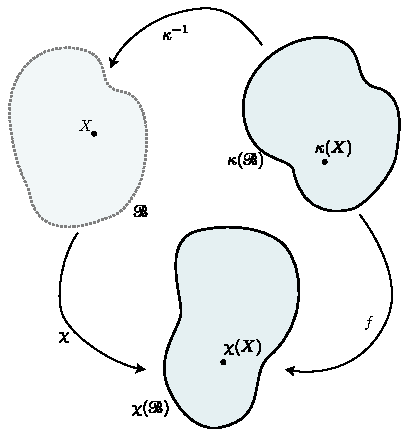
\includegraphics[scale=1.2]{figure/cinematica/def3d}
	\caption{Deformazione $f$.}
	\label{fig:def3d}
\end{figure}





\subsection{Gradiente della deformazione}
Come già fatto in precedenza, assumeremo $\fb$ e $\fb^{-1}$ continue e differenziabili. Trovandoci adesso in un ambiente tridimensionale, per desumere l'effetto locale della deformazione, occorre esplorarne un intorno in una certa direzione $\hb\in \Vc$, la cui lunghezza $|\hb|$ che faremo tendere a zero. Questa operazione definirà la derivata direzionale di $\fb$, esprimibile in termini del \textit{gradiente di deformazione} $\nabla\fb\equiv\Fb$ secondo la definizione:
\begin{definition}
\begin{equation}
	\lim_{\hb\to\mathbf{0}}\frac{\fb(\xb+\hb)-\fb(\xb)}{|\hb|}=:\Fb(\xb)\hb.
\end{equation}
\end{definition}

Questa relazione si può facilmente riscrivere come
\begin{equation}
\fb(\xb+\hb)-\fb(\xb)=\Fb(\xb)\hb+o(|\hb|).
\end{equation}
Dunque, a meno di infinitesimi di ordine superiore a $|\hb|$, il vettore $\xb+\hb-\xb=\hb$ viene mandato in $\Fb(\xb)\hb$.

Se $\{\eb_i\}$ è una base cartesiana, allora è possibile scrivere il gradiente della deformazione come
\begin{equation}
	\Fb=\fb,_{i}\otimes\eb_i.
\end{equation}

Nel contesto monodimensionale abbiamo assunto che  $f'(x)$ fosse strettamente positiva, il che implicava la preservazione dell'orientazione dello spazio. L'analoga richiesta nel caso tridimensionale si traduce nella pretesa che
\begin{equation}\label{detpos}
	\det \Fb(\xb)>0 \qquad\forall \xb\in\Omega.
\end{equation}

L'interpretazione fisica della \eqref{detpos} è facilmente deducibile se si ricorda la definizione di determinante di un tensore del secondo ordine $\Ab\in\Lin$: dati tre vettori $\ub, \vb,\wb\in \Vc$ non collineari, il determinante di $\Ab$ è il numero 
\begin{equation}\label{det}
	\det \Ab\coloneqq \frac{\Ab\ub\times\Ab\vb\cdot\Ab\wb}{\ub\times\vb\cdot\wb}.
\end{equation}
Il denominatore del membro destro di \eqref{det} è il volume con segno (positivo se la terna $\ub, \vb,\wb$ è positivamente orientata) del parallelepipedo di spigoli  $\ub, \vb,\wb$, mentre il numeratore  rappresenta il volume con segno del parallelepipedo di spigoli $\Ab\ub, \Ab\vb,\Ab\wb$, ovvero le immagini della terna di vettori originaria sotto l'applicazione $\Ab$. In particolare, se $\Ab=\Fb$, il numeratore rappresenta allora il volume del parallelepipedo deformato per effetto di $\fb$. Dunque se $\det \Fb(\xb)$ fosse nullo, vorrebbe dire che il parallelepipedo originario si è contratto in un punto, evenienza che vogliamo scongiurare; inoltre, se fosse negativo, significherebbe che l'orientazione della terna originaria sarebbe cambiata, circostanza che desideriamo parimenti evitare.

Scriviamo adesso in esplicito le componenti del gradiente di deformazione. Per definizione abbiamo:
\begin{equation}
	\begin{aligned}
	F_{ij}=(\Fb\eb_j)\cdot \eb_i=\fb_{,j}\cdot \eb_i=f_{i,j}.
	\end{aligned}
\end{equation}
La matrice che rappresenta $\Fb$ nella base ${\eb_i}$ è allora
\begin{equation}
[\Fb]=
\begin{bmatrix}
	f_{1,1}&f_{1,2}&f_{1,3}\\f_{2,1}&f_{2,2}&f_{2,3}\\f_{3,1}&f_{3,2}&f_{3,3}
\end{bmatrix}.
\end{equation}

\begin{exercise}
Data la deformazione $\fb(\xb)=\xb+\alpha x_2\eb_2+\beta x_2x_3\eb_3$, con $\xb=x_1\eb_1+x_2\eb_2+x_3\eb_3$. Determinare il gradiente di deformazione.
\begin{svolgimento}
Le componenti della deformazione sono:
\begin{equation}
\begin{aligned}
	&f_{1}=\fb\cdot \eb_{1}=x_{1},\\
	&f_{2}=\fb\cdot \eb_{2}=x_{2}+\alpha x_{2},\\
	&f_{3}=\fb\cdot \eb_{3}=x_{3}+\beta x_{2}x_{3},\end{aligned}
\end{equation}
da cui si ricava immediatamente
\begin{equation}
	[\Fb]=
	\begin{bmatrix}
		f_{1,1}&f_{1,2}&f_{1,3}\\f_{2,1}&f_{2,2}&f_{2,3}\\f_{3,1}&f_{3,2}&f_{3,3}
	\end{bmatrix}=
	\begin{bmatrix}
	1&0&0\\0&1+\alpha&0\\0&\beta x_3&1+\beta x_2
	\end{bmatrix}.
\end{equation}
Senza ricorrere alla rappresentazione matriciale, si ricava subito:
\begin{equation}
\Fb=\fb_{,i}\otimes\eb_i=\eb_1\otimes\eb_1+(1+\alpha)\eb_2\otimes\eb_2+\beta x_3\eb_3\otimes\eb_2+(1+\beta x_2)\eb_3\otimes\eb_3.
\end{equation}
\end{svolgimento}
\end{exercise}


\subsection{Spostamento}
Se $\xb$ e $\fb(\xb)$ sono, rispettivamente, la posizione occupata da un punto materiale in due piazzamenti, la differenza tra i due definisce il vettore spostamento:
\begin{definition}
\begin{equation}
	\ub(\xb)\coloneqq\fb(\xb)-\xb.
\end{equation}
\end{definition}

\begin{figure}
	\centering
	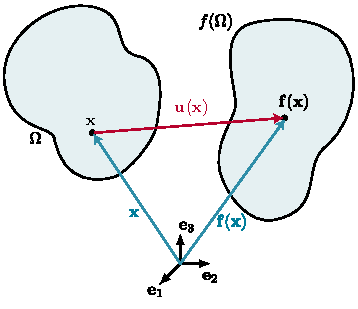
\includegraphics[scale=1.2]{figure/cinematica/displ}
	\caption{Vettore spostamento.}
	\label{fig:displ}
\end{figure}




Il suo gradiente, che indicheremo con $\Hb\coloneqq\nabla\ub$, è allora

\begin{definition}
	\begin{equation}\label{HFI}
	\Hb(\xb)=\Fb(\xb)-\Ib,
\end{equation}
\end{definition}
dove $\Ib$ è il tensore identità. Se $\{\eb_i\}$ è una base cartesiana, allora
\begin{equation}
\Hb=\ub,_i\otimes\eb_i
\end{equation}
e le componenti di $\Hb$ si trovano immediatamente come:
\begin{equation}
	H_{ij}=\Hb\eb_j\cdot\eb_i=u_{i,j}.
\end{equation}


\section{Variazione di lunghezza}
Consideriamo, in una configurazione di riferimento, due punti `prossimi' $\xb$  e $\xb_0$. Il segmento `infintesimo' che essi individuano ha lunghezza
\begin{equation}
d\ell_0=|\xb-\xb_0|.
\end{equation}
Denotando con $\tb$ il versore che individua la direzione
\begin{equation}
\tb\coloneqq\frac{\xb-\xb_0}{|\xb-\xb_0|},
\end{equation}
allora
\begin{equation}
\xb-\xb_0=d\ell_0 \tb.
\end{equation}
Le immagini di $\xb$  e $\xb_0$ a seguito della deformazione sono $\fb(\xb)$ e $\fb(\xb_0)$ , che individuano un segmento di lunghezza
\begin{equation}
	d\ell:=|\mathbf{f}(\mathbf{x})-\mathbf{f}(\mathbf{x}_0)|.
\end{equation}

\begin{center}
	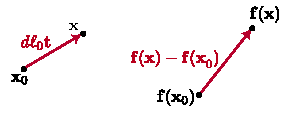
\includegraphics[scale=1.2]{figure/cinematica/dl}
\end{center}

Espandendo in serie di Taylor la deformazione attorno al punto $\xb_0 $ si ha
\begin{equation}
	\mathbf{f}(\mathbf{x})=\mathbf{f}(\mathbf{x}_{0})+\mathbf{F}(\mathbf{x}_{0})[\mathbf{x-x}_{0}]+o(|\mathbf{x-x}_{0}|),
\end{equation}
ovvero
\begin{equation}
	\mathbf{f}(\mathbf{x})-\mathbf{f}(\mathbf{x}_0)=d\ell_0\mathbf{F}\mathbf{t}+o(d\ell_0),
\end{equation}
da cui 
\begin{equation}
	d\ell=|\mathbf{f}(\mathbf{x})-\mathbf{f}(\mathbf{x}_0)|=d\ell_0|\mathbf{F}\mathbf{t}|+o(d\ell_0).
\end{equation}
Ne segue che, a meno di infinitesimi di ordine $o(d\ell_0)$, il rapporto tra le due lunghezze vale
\begin{definition}
\begin{equation}\label{dl}
	\frac{d\ell}{d\ell_0}=|\mathbf{Ft}|.
\end{equation}
\end{definition}


Abbiamo dunque concluso che, dato  un segmento infinitesimo in direzione $\tb$ nella configurazione di riferimento, il rapporto tra la lunghezza del segmento deformato e la lunghezza del segmento indeformato è uguale al modulo del gradiente di deformazione applicato a $\tb$.

Osserviamo adesso che $|\mathbf{Ft}|$ può essere riscritto come
\begin{equation}
	|\mathbf{Ft}|=\sqrt{\Fb\tb\cdot\Fb\tb}=\sqrt{\Fb^\top\Fb\tb\cdot\tb}.
\end{equation}
Introducendo il \textit{tensore destro di Cauchy-Green}
\begin{definition}
	\begin{equation}
\Cb\coloneqq\Fb^\top\Fb,
\end{equation}
\end{definition}
il rapporto tra la lunghezza del segmento deformato e la lunghezza del segmento indeformato può essere scritto in alternativa come
\begin{equation}
	\frac{d\ell}{d\ell_0}=\sqrt{\Cb\tb\cdot\tb}.
\end{equation}

\begin{remark}
Risulta interessante osservare che $\Cb^\top=(\Fb^\top\Fb)^\top=\Fb^\top\Fb=\Cb$ e dunque $\Cb$ è simmetrico.  Questa circostanza suggerisce che per valutare la variazione di lunghezza non è necessario conoscere tutto il gradiente di deformazione $\Fb$, che ha in generale nove componenti, ma è sufficiente conoscere $\Cb$, che si caratterizza con sei componenti. Questo suggerisce che il gradiente della deformazione $\Fb$ include maggiore informazione rispetto a $\Cb$, ma questa non è necessaria per caratterizzare le variazioni di lunghezza. Non è difficile intuire che l'informazione aggiuntiva riguarda la componente rigida della deformazione, come vedremo più avanti.
\end{remark}


\section{Deformazioni omogenee}
Una deformazione è \textit{omogenea} se il suo gradiente è costante. In particolare vale la seguente rappresentazione:
\begin{definition}
	\begin{equation}
	\fb(\xb)=\fb(\xb_0)+\Fb(\xb-\xb_0),
\end{equation}
\end{definition}
con $\Fb$ costante. Sono esempi di deformazioni omogenee le \textit{traslazioni}:
\begin{equation}
	\fb(\xb)=\xb +\cb,
\end{equation}
con $\cb$ costante. In questa deformazione ogni punto viene traslato del vettore $\cb$.

Un altro esempio rilevante è costituito dalle rotazioni, ovvero deformazioni del tipo
\begin{equation}
	\fb(\xb)=\xb_0+\Rb(\xb-\xb_0),
\end{equation}
con $\Rb\in\Rot$ e $\xb_0\in\Vc$; con questa deformazione il corpo viene ruotato attorno al punto $\xb_0$, come stabilito dal tensore ortogonale $\Rb$.

\begin{exercise}
	Dato un sistema di riferimento cartesiano $\{\eb_i\}$, si consideri  l'effetto della rotazione attorno all'asse $\eb_3$ per l'origine sui vettori della base.
	
	\begin{svolgimento}
		La deformazione in questione è omogenea ed è data da
		\begin{equation}
			\fb(\xb)=\Rb\xb,
		\end{equation}
	il cui gradiente vale $\Fb=\Rb$. La matrice rappresentativa della rotazione data è
		\begin{equation}\label{Rp}
			[\Rb]=\begin{bmatrix}\cos\theta&-\sin\theta&0\\\sin\theta&\cos\theta&0\\0&0&1\end{bmatrix}.
		\end{equation}
È allora immediato verificare quale sia l'effetto sui vettori della base:
\begin{equation}
\Fb\eb_1=\Rb\eb_1=\cos\theta\eb_1-\sin\theta\eb_2, \quad \Fb\eb_2=\Rb\eb_2=\sin\theta\eb_1+\cos\theta\eb_2,  \quad 
\Fb\eb_3=\Rb\eb_3=\eb_3.
\end{equation}
	\end{svolgimento}
\end{exercise}

Una deformazione è \textit{rigida} se  lascia inalterate le distanze mutue tra i punti, ovvero
\begin{equation}\label{fxfz}
	|\mathbf{f}(\mathbf{x})-\mathbf{f}(\mathbf{z})|=|\mathbf{x}-\mathbf{z}|\quad\forall\mathbf{x},\mathbf{z}\in\Omega.
\end{equation}
Vediamo qual è la conseguenza di questa circostanza. 

Prima di farlo, troviamo  un risultato utile nel seguente esercizio.

\begin{exercise}\label{gradab}
Siano $\ab(\xb)$ e $\bb(\xb)$ due campi vettoriali. Determinare il gradiente di $\ab(\xb)\cdot\bb(\xb)$.

\begin{svolgimento}
Il gradiente che cerchiamo è
\begin{equation}
\nabla\big( \ab(\xb)\cdot\bb(\xb) \big)=\partial_\xb\big( \ab(\xb)\cdot\bb(\xb) \big).
\end{equation}
Conviene lavorare per componenti. Omettendo la dipendenza dei campi da $\xb$, si ha 
\begin{equation}
	\begin{aligned}
\nabla\big( \ab\cdot\bb\big)=\partial_\xb\big( \ab\cdot\bb \big)&=(a_i b_i),_{j}=a_{i,j}b_i+a_ib_{i,j}=(a_{j,i})^\top b_i+(b_{j,i})^\top a_i\\
&=(\nabla\ab)^\top\bb+(\nabla \bb)^\top\ab.
\end{aligned}
\end{equation}
\end{svolgimento}
	
\end{exercise}


La \eqref{fxfz} è equivalente a richiedere
\begin{equation}
	\left(\mathbf{f}(\mathbf{x})-\mathbf{f}(\mathbf{z})\right)\cdot\left(\mathbf{f}(\mathbf{x})-\mathbf{f}(\mathbf{z})\right)=(\mathbf{x}-\mathbf{z})\cdot(\mathbf{x}-\mathbf{z})\quad\forall\mathbf{x},\mathbf{z}\in\Omega.
\end{equation}
Derivando rispetto a $\xb$, utilizzando il risultato dell'esercizio \ref{gradab}, si trova
\begin{equation}
2	\Fb^\top(\xb)\fb(\xb)-2\Fb^\top(\xb)\fb(\zb)=2\xb-2\zb  \quad\forall\mathbf{x},\mathbf{z}\in\Omega;
\end{equation}
derivando adesso rispetto a $\zb$ si ricava
\begin{equation}
\Fb^\top(\xb)\Fb(\zb)=\Ib.
\end{equation}
Questo significa che $\Fb$ non dipende dal punto ed è un tensore ortogonale. Ma dato che $\det\Fb>0$, segue che è una rotazione.

Concludiamo allora che le deformazioni rigide hanno la seguente rappresentazione generale:
\begin{definition}
	\begin{equation}
	\begin{aligned}\mathbf{f}(\mathbf{x})&=\mathbf{f}(\mathbf{x}_0)-\mathbf{x}_0&&\text{traslazione del generico punto }\mathbf{x}_0,\\&+\mathbf{x}_0+\mathbf{Q}[\mathbf{x}-\mathbf{x}_0]&&\text{rotazione attorno al punto }\mathbf{x}_0,\end{aligned}
\end{equation}
\end{definition}
con $\Qb \in \Rot$.
In altri termini una deformazione rigida è data dalla composizione di una traslazione con una rotazione (ovvero una \textit{rototraslazione}).


\section{Misure di deformazione}
Abbiamo già osservato che, per misurare le variazioni di lunghezza, non è necessario conoscere l'intero gradiente di deformazione $\Fb$, che ha in generale 9 componenti, ma basta il tensore  destro di Cauchy-Green $\Cb$. Abbiamo anche visto che $\Cb$ è simmetrico ed è immediato verificare che è anche definito positivo.\footnote{Infatti, preso un qualunque $\ab\in\Vc$
\begin{equation}
\Cb \ab\cdot\ab=\Fb \ab\cdot\Fb\ab=|\Fb\ab|^2\geq 0.
	\end{equation}
Inoltre $\Cb \ab\cdot\ab=0$ se e solo se $|\Fb \ab|=0$ e questo è vero se e solo se $\Fb \ab=\mathbf{0}$; ma $\det \Fb >0$, quindi $\Fb\ab=\mathbf{0}$ se e solo se $\ab=\mathbf{0}$. Pertanto
\begin{equation}
	\Cb \ab\cdot\ab>0 \quad \forall \ab\neq\mathbf{0}.
\end{equation}
}
Per il teorema spettrale $\Cb$ può allora essere rappresentato come
\begin{equation}
\Cb =\sum_{i=1}^3\lambda_i \cb_i\otimes\cb_i,
\end{equation}
dove   gli autovalori $\lambda_i$ sono  positivi. Possiamo quindi definire il tensore
\begin{equation}
\Ub\coloneqq \sum_{i=1}^3\sqrt{\lambda_i }\cb_i\otimes\cb_i,
\end{equation}
ovvero $\Cb=\Ub\Ub=\Ub^2$. Il tensore $\Ub$, detto \textit{tensore destro della deformazione}, è ovviamente simmetrico e definito positivo ed è la somma di tre estensioni in tre direzioni ortogonali. Definiamo
\begin{equation}
\Rb=\Fb\Ub^{-1}.
\end{equation}
Il tensore $\Rb$ è chiaramente una rotazione. Infatti
\begin{equation}
	\mathbf{R}^\top\mathbf{R}=\mathbf{U}^{-1}\mathbf{F}^\top\mathbf{F}\mathbf{U}^{-1}=\mathbf{U}^{-1}\mathbf{C}\mathbf{U}^{-1}=\mathbf{U}^{-1}\mathbf{U}\mathbf{U}\mathbf{U}^{-1}=\mathbf{I}.
\end{equation}

Vale quindi la seguente decomposizione, chiamata \textit{decomposizione polare},
\begin{definition}
	\begin{equation}\label{polar}
\Fb=\Rb \Ub.
\end{equation}
\end{definition}
dove $\Rb$ è una rotazione e $\Ub$ una deformazione pura (v. Fig. \ref{fig:polar}). La rappresentazione \eqref{polar} mostra quindi in maniera evidente che $\Fb$ contiene in sé una parte che è una rotazione e dunque non responsabile di variazioni di lunghezze.
%
\begin{figure}[h!]
	\centering
	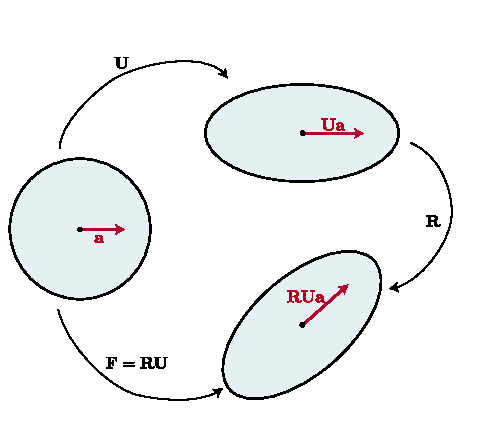
\includegraphics[scale=1.2]{figure/cinematica/polar}
	\caption{Effetto della decomposizione polare. L'azione di $\Fb$ sul vettore $\ab$ può essere decomposta come l'azione di una deformazione pura $\Ub$ seguita da una rotazione $\Rb$.}
\label{fig:polar}
\end{figure}
%
In questo senso $\Fb$ \textit{non} è una buona \textit{misura di deformazione}. I tensori $\Cb$ e $\Ub$ sono invece idonei a descrivere i cambiamenti di forma dei corpi associati a variazioni metriche. Tuttavia essi non si annullano in corrispondenza di deformazioni rigide. Infatti se $\Fb=\Rb$, risulta che $\Cb =\Ub=\Ib$.  Poiché ha senso definire la misura di deformazione come un difetto di rigidità, introduciamo il tensore di \textit{Green--Saint-Venant}
\begin{definition}
	\begin{equation}
\Db\coloneqq\frac{1}{2}(\Cb -\Ib),
\end{equation}
\end{definition}
che fa corrispondere ad una deformazione rigida il tensore nullo. Il fattore $1/2$ non ha un significato fisico, ma risulterà comodo nel seguito.


\begin{exercise}
Sia assegnato il seguente gradiente di deformazione:
\begin{equation}
\Fb=-\frac{1}{2}(\alpha+\beta)\eb_1\otimes\eb_1+\frac{1}{2}(\alpha-\beta)\eb_2\otimes\eb_2-\frac12 (\alpha+\beta)(\eb_1\otimes\eb_2-\eb_2\otimes\eb_1)+\gamma \,\eb_3\otimes\eb_3,
\end{equation}
con $\alpha,\beta$ e $\gamma$ costanti positive. Determinare la decomposizione polare di  $\Fb$.
\begin{svolgimento}
La rappresentazione matriciale di $\Fb$ è 
\begin{equation}
[\Fb]=	\left[
\begin{array}{ccc}
	-\dfrac{ \alpha+\beta }{2} & -\dfrac{1}{2} (\alpha +\beta ) & 0 \\ [.2cm]
	\dfrac{\alpha +\beta }{2} & \dfrac{\alpha -\beta }{2} & 0 \\[.2cm]
	0 & 0 & \gamma  \\
\end{array}.
\right]
\end{equation}
Un semplice calcolo mostra che la matrice rappresentativa del tensore destro di Cauchy-Gren $\Cb=\Fb^\top\Fb$ è
\begin{equation}
[\Cb]=\left[
\begin{array}{ccc}
	\dfrac{1}{2} \left(\alpha ^2+\beta ^2\right) & \dfrac{1}{2} (\alpha -\beta ) (\alpha
	+\beta ) & 0 \\[.2cm]
	\dfrac{1}{2} (\alpha -\beta ) (\alpha +\beta ) & \dfrac{1}{2} \left(\alpha ^2+\beta
	^2\right) & 0 \\[.2cm]
	0 & 0 & \gamma ^2 \\
\end{array}.
\right]
\end{equation}
Determiniamo gli autovalori di $\Cb$, soluzione del polinomio caratteristico
\begin{equation}
	\det(\Cb-\lambda \Ib)=\left(\gamma ^2-\lambda \right) \left(\alpha ^2 \beta ^2-\alpha ^2 \lambda -\beta ^2
	\lambda +\lambda ^2\right),
\end{equation}
le cui soluzioni sono
\begin{equation}
\lambda_1=\alpha^2, \quad \lambda_2=\beta^2, \quad \lambda_3=\gamma^2.
\end{equation}
I corrispondenti autovettori risultano
\begin{equation}
\cb_1=\frac{1}{\sqrt{2}}(\eb_1+\eb_2), \quad \cb_2=\frac{1}{\sqrt{2}}(-\eb_1+\eb_2), \quad \cb_3=\eb_3.
\end{equation}
La rappresentazione spettrale di $\Cb$ è dunque
\begin{equation}
\Cb=\alpha^2 \, \cb_1\otimes\cb_1+\beta^2 \, \cb_2\otimes\cb_2+\gamma^3\eb_3\otimes\eb_3,
\end{equation}
e quindi
\begin{equation}
	\Ub=\alpha \, \cb_1\otimes\cb_1+\beta \, \cb_2\otimes\cb_2+\gamma\eb_3\otimes\eb_3.
\end{equation}
L'inversa di $\Ub$ si trova immediatamente:
\begin{equation}
\Ub^{-1}=\frac{1}{\alpha} \, \cb_1\otimes\cb_1+\frac{1}{\beta} \, \cb_2\otimes\cb_2+\frac{1}{\gamma} \eb_3\otimes\eb_3,
\end{equation}
ovvero, ricordando l'espressione degli autovettori
\begin{equation}
\Ub^{-1}=\left[
\begin{array}{ccc}
	\dfrac{\alpha +\beta }{2 \alpha  \beta } & \dfrac{1}{2} \left(\dfrac{1}{\alpha
	}-\dfrac{1}{\beta }\right) & 0 \\[.2cm]
	\dfrac{1}{2} \left(\dfrac{1}{\alpha }-\dfrac{1}{\beta }\right) & \dfrac{\alpha +\beta }{2
		\alpha  \beta } & 0 \\[.2cm]
	0 & 0 & \dfrac{1}{\gamma } \\
\end{array}
\right].
\end{equation}
Il tensore di rotazione ha allora come matrice rappresentativa
\begin{equation}
[\Rb]=[\Fb][\Ub^{-1}]=\left[
\begin{array}{ccc}
	0 & -1 & 0 \\
	1 & 0 & 0 \\
	0 & 0 & 1 \\
\end{array}
\right],
\end{equation}
ovvero 
\begin{equation}
	\Rb=-\eb_1\otimes\eb_2+\eb_2\otimes\eb_1+\eb_{3}\otimes\eb_{3}.
\end{equation}
Confrontando con la \eqref{Rp}, si vede facilmente che $\Rb$ rappresenta una rotazione di $\pi/2$ attorno all'asse $\eb_3$. 

	Concludiamo che il gradiente di deformazione assegnato consiste in una dilatazione di $\alpha$ nella direzione di $\cb_1$, una dilatazione di $\beta$ nella direzione di $\cb_2$, una dilatazione di $\gamma$ in direzione $\cb_3$ e una rotazione di $\pi/2$ attorno a $\eb_3$.
\end{svolgimento}
\end{exercise}


\begin{exercise}
	Sia dato il campo di spostamenti
	%Libro Capecchi
	\begin{equation}
		\ub(\xb)=\frac{3}{L}x_1^2\eb_1+\frac{2}{L^2}x_2x_3^2\eb_2+\frac{1}{L^2}x_1x_3^2\eb_3.
	\end{equation}
	\begin{enumerate}
		\item Determinare la posizione del punto $P$ che prima della deformazione occupava la posizione $\xb=L\eb_1+2L\eb_3$.
		\item Determinare la deformazione $\fb(\xb)$, il gradiente della deformazione $\Fb(\xb)$, il gradiente dello spostamento $\Hb(\xb)$, il tensore destro di Cauchy--Green $\Cb(\xb)$ e il tensore della deformazione di Green--Saint-Venant $\Db(\xb)$ nel punto $P$.
		\item Stabilire se la deformazione è omogenea.
		\item Calcolare la variazione di lunghezza relativa $dl/dl_0$ nella direzione $\eb_1$ e la variazione di volume relativa $dv/dv_0$ nel punto $P$.
	\end{enumerate}
	\begin{svolgimento}
		\begin{enumerate}
			\item La deformazione si trova facilmente come
			\begin{equation}
				\fb(\xb)=\ub(\xb)+\xb=\left(x_1+\frac{3}{L}x_1^2\right)\eb_1+\left(x_2+\frac{2}{L^2}x_2x_3^2\right)\eb_2+\left(x_3+\frac{1}{L^2}x_1x_3^2\right)\eb_3.
			\end{equation}
			Dunque la posizione del punto $P$ dopo la deformazione risulta essere
			\begin{equation}
				\yb(P)=\fb{(\xb(P))}=2L(2\eb_1+3\eb_3).
			\end{equation}
			\item
			Usando la definizione, si ha che
			\begin{equation}
				\begin{aligned}
					\Fb(\xb)&=\fb{,_i}\otimes\eb_i=\left(1+\frac{6x_1}{L}\right)\eb_1\otimes\eb_1+\frac{x_3^2}{L^2}\eb_3\otimes\eb_1+\left(1+\frac{2x_3^2}{L^2}\right)\eb_2\otimes\eb_2\\
					&+\frac{4x_2x_3}{L^2}\eb_2\otimes\eb_3+\left(1+\frac{2x_1x_3}{L^2}\right)\eb_3\otimes\eb_3.
				\end{aligned}
			\end{equation}
			Si può d'altra parte ragionare per componenti, ricordando che $F_{ij}=f_{i,j}$,\footnote{Si ricorda che con $f_{i,j}$ si intende $\frac{\partial f_i}{\partial x_j}$.} per ottenere la matrice rappresentativa di $\Fb$:
			\begin{equation}
				[\Fb(\xb)]=\left[\begin{matrix}
					1+\frac{6x_1}{L}&0&0\\
					0&1+\frac{2x_3^2}{L^2}&\frac{4x_2x_3}{L^2}\\
					\frac{x_3^2}{L^2}&0&1+\frac{2x_1x_3}{L^2}
				\end{matrix}\right].
			\end{equation}
			Valutando $\Fb$ nel punto $P$, si ha
			\begin{equation}
				\Fb(\xb(P))=7\eb_1\otimes\eb_1+9\eb_2\otimes\eb_2+4\eb_3\otimes\eb_1+5\eb_3\otimes\eb_3.
			\end{equation}
			Analogamente si procede per $\Hb(\xb)$, ovvero, una volta calcolata $\Fb(\xb)$, basta ricordare che $\Hb=\Fb-\Ib$:
			\begin{equation}
				\Hb( \xb)=\left(\frac{6x_1}{L}\right)\eb_1\otimes\eb_1+\frac{x_3^2}{L^2}\eb_3\otimes\eb_1+\left(\frac{2x_3^2}{L^2}\right)\eb_2\otimes\eb_2+\frac{4x_2x_3}{L^2}\eb_2\otimes\eb_3+\left(\frac{2x_1x_3}{L^2}\right)\eb_3\otimes\eb_3.
			\end{equation}
			%
			Infine, si determina il tensore destro di Cauchy--Green:
			\begin{equation}
				\Cb(\xb(P))=65\eb_1\otimes\eb_1+20(\eb_1\otimes\eb_3+\eb_3\otimes\eb_2)+81\eb_2\otimes\eb_2+25\eb_3\otimes\eb_3
			\end{equation}
			e il tensore di Green--Saint-Venant:
			\begin{equation}
				\Db(\xb(P))=\frac12(\Cb(\xb(P))-\Ib)=\Big( 32\eb_1\otimes\eb_1+10(\eb_1\otimes\eb_3+\eb_3\otimes\eb_2)+40\eb_2\otimes\eb_2+12\eb_3\otimes\eb_3 \Big).
			\end{equation}
			\item Dato che $\Fb(\xb)$ non è costante, la deformazione non è omogenea.
			\item La variazione relativa di lunghezza nel punto $P$ e nella direzione $\eb_1$ è
			\begin{equation}
				\frac{d\ell}{d\ell_0}=|\Fb(\xb(P))\eb_1|=\sqrt{65},
			\end{equation}
			mentre la variazione relativa di volume
			\begin{equation}
				\frac{dv}{dv_0}=\det\big(\Fb(\xb(P))\big)=315.
			\end{equation}
		\end{enumerate}
	\end{svolgimento}
\end{exercise}

\begin{exercise}
	Sia $\rb\,:\,[0,2\pi]\mapsto\Omega$ l'elica cilindrica parametrizzata da
	\begin{equation}
		\rb(\theta)=\cos\theta\eb_1+\sin\theta\eb_2+\theta\eb_3
	\end{equation}
	ed $\fb$ la deformazione
	\begin{equation}
		\fb(\xb)=x_2\eb_1+x_1\eb_2+2 x_3\eb_3.
	\end{equation}
	\begin{enumerate}
		\item Determinare il gradiente di deformazione $\Fb(\xb)$ e il tensore destro di Cauchy--Green $\Cb(\xb)$.
		\item Calcolare le lunghezze $\ell_0$, dell'elica indeformata, ed $\ell$, dell'elica deformata.
	\end{enumerate}
	
	\begin{svolgimento}
		\begin{enumerate}
			\item Applicando la definizione, si calcola subito
			\begin{equation}
				\Fb(\xb)=\fb,_{i}(\xb)\otimes\eb_i=\eb_2\otimes\eb_1+\eb_1\otimes\eb_2+2\eb_3\otimes\eb_3.
			\end{equation}	
			D'altra parte, utilizzando la rappresentazione per componenti e ricordando che $F_{ij}=f_{i,j}$, si trova che
			\begin{equation}
				[\Fb]=\left[   
				\begin{matrix}
					0&1&0	\\
					1&0&0\\
					0&0&2
				\end{matrix}
				\right]\end{equation}
			Trovare il tensore di Cauchy-Green è immediato:
			\begin{equation}
				\Cb=\Fb^\top\Fb=\eb_1\otimes\eb_1+\eb_2\otimes\eb_2+4\eb_3\otimes\eb_3, 
			\end{equation}
			ovvero
			\begin{equation}
				[\Cb]=[\Fb^\top\Fb]=\left[
				\begin{matrix}
					1&0&0\\
					0&1&0\\
					0&0&4
				\end{matrix}
				\right].
			\end{equation}
			
			
			
			\item Il generico punto  dell'elica è dato da $\rb(\theta)$, al variare di $\theta\in[0,2\pi]$. Per ottenere la lunghezza iniziale dell'elica, è sufficiente utilizzare la formula per calcolare la lunghezza di una curva:
			\begin{equation}
				\ell_0=\int_0^{2\pi}|\rb'(\theta)|d\theta=2\sqrt{2}\pi.
			\end{equation}
			Per effetto della deformazione, il generico punto  dell'elica viene mandato in
			\begin{equation}
				\yb=\fb\big(\rb(\theta)\big)=\sin\theta\eb_1+\cos\theta\eb_2+2\theta\eb_3.
			\end{equation}
			La lunghezza dell'elica deformata è allora
			\begin{equation}
				\ell=\int_0^{2\pi}|\yb'(\theta)|d\theta=2\sqrt{5}\pi.
			\end{equation}
		\end{enumerate}
	\end{svolgimento}
	
\end{exercise}



\section{Teoria infinitesima}


Dalla \eqref{dl}, si evince che, se il gradiente di deformazione è prossimo all'identità, allora le variazioni di lunghezza sono piccole. Possiamo dunque introdurre un parametro di piccolezza, dato da
\begin{equation}
	\varepsilon\coloneqq\sup_{\xb\in\Omega}|\Fb(\xb)-\Ib|,
\end{equation}
che misura la maggiore distanza tra $\Fb$ e l'identità. Vista la definizione di gradiente di spostamento e la \eqref{HFI}, il parametro può essere riscritto come
\begin{equation}\label{eps}
\varepsilon=\sup_{\xb\in\Omega}|\Hb(\xb)|.
\end{equation}

Vogliamo adesso considerare una teoria, detta appunto \textit{infinitesima}, ottenuta trascurando infinitesimi di ordine superiore al primo di $\varepsilon$.

\subsection{Il tensore della deformazione infinitesima}
Vediamo innanzitutto quali (o quale?) siano le misure di deformazione in teoria infinitesima. Osserviamo  che possiamo scrivere il gradiente della deformazione come
\begin{equation}
\Fb(\xb)=\Ib +\varepsilon(\xb) \widetilde{\Hb}(\xb), \qquad \varepsilon(\xb)\coloneqq |\Hb(\xb)|, \quad \widetilde{\Hb}(\xb)\coloneqq \frac{\Hb(\xb)}{|\Hb(\xb)|}.
\end{equation}
Vista la \eqref{eps}, senz'altro
\begin{equation}
\varepsilon(\xb)\leq \varepsilon \qquad \forall \xb\in \Omega
\end{equation}
e dunque saremo autorizzati a trascurare i termini dell'ordine di $\varepsilon^2(\xb)$. Trascurando tali termini, Il tensore destro di Cauchy-Green diventa allora
\begin{equation}\label{Cap}
	\begin{aligned}
	\Cb(\xb)=	\mathbf{F}^\top(\mathbf{x})\mathbf{F}(\mathbf{x})& =\mathbf{I+H^\top(x)+H(x)+\frac12H^\top(x)H(x)}  \\
		&=\mathbf{I}+\varepsilon(\mathbf{x})\widetilde{\mathbf{H}}^\top(\mathbf{x})+\varepsilon(\mathbf{x})\widetilde{\mathbf{H}}(\mathbf{x})+\frac12\varepsilon^2(\mathbf{x})\widetilde{\mathbf{H}}^\top(\mathbf{x})\widetilde{\mathbf{H}}(\mathbf{x}) \\
		&=\mathbf{I}+\varepsilon(\mathbf{x})\widetilde{\mathbf{H}}^\top(\mathbf{x})+\varepsilon(\mathbf{x})\widetilde{\mathbf{H}}(\mathbf{x}) \\
		&=\mathbf{I+H^\top(x)+H(x)}.
	\end{aligned}
\end{equation}
Nel seguito eviteremo d’introdurre il parametro $\varepsilon$ e trascureremo i termini
superlineari in $\Hb$
.
La misura di deformazione di Green--Saint-Venant diventa dunque
\begin{equation}
\Db(\xb)=\frac{1}{2}(\Cb(\xb)-\Ib)=\frac{1}{2}\left(\mathbf{H(x)+H^\top(x)}\right).
\end{equation}
Il tensore 
\begin{definition}
	\begin{equation}\label{simgrad}
	\Eb(\xb)\coloneqq\sym \Hb(\xb)
\end{equation}
\end{definition}
è detto \textit{tensore della deformazione infinitesima}, che servirà a caratterizzare completamente le variazioni metriche in teoria infinitesima.

\subsection{Il tensore della rotazione infinitesima }
Come qualunque tensore del secondo ordine, il gradiente dello spostamento può essere decomposto nella sua parte simmetrica e antisimmetrica:
\begin{equation}
	\Hb=\sym \Hb+\skw \Hb.
\end{equation}
Abbiamo già definito il tensore della deformazione infinitesima $\Eb=\sym \Hb$; mostriamo adesso che la parte antisimmetrica
\begin{definition}
	\begin{equation}
\Wb\coloneqq\skw \Hb
\end{equation}
\end{definition}
rappresenta una rotazione rigida infinitesima. Per farlo, approssimiamo la relazione
\begin{equation}
\Rb=\Fb\Ub^{-1}
\end{equation}
per vedere com'è fatta una rotazione infinitesima. Trascurando i termini superlineri in $\Hb$, dalla \eqref{Cap} segue che
\begin{equation}
\Ub^2=\Cb=\Ib+2\Eb.
\end{equation}
D'altra parte vale la seguente catena di uguaglianze:
\begin{equation}
(\Ib+\Eb)^2=(\Ib+\Eb)(\Ib+\Eb)=\Ib+2\Eb=\Ub^2,
\end{equation}
da cui possiamo dedurre che 
\begin{equation}
	\Ub=\Ib+\Eb.
\end{equation}
Avendo adesso l'approssimazione per $\Ub$, è necessario trovare quella per $\Ub^{-1}$.  Poiché
\begin{equation}
(\Ib+\Eb)(\Ib-\Eb)=\Ib,
\end{equation}
possiamo concludere che
\begin{equation}
\Ub^{-1}=\Ib-\Eb.
\end{equation}
Siamo dunque pronti per determinare la forma che assume una rotazione $\Rb$ quando si trascurino i termini superlineari in $\Hb$ (ovvero in piccole deformazioni):
\begin{equation}
\Rb=\Fb\Ub^{-1}=(\Ib+\Hb)(\Ib-\Eb)=\Ib-\Eb+\Hb=\Ib+\Wb.
\end{equation}
Concludiamo allora che la rotazione di un punto $\xb$ attorno a $\xb_0$ ha la seguente rappresentazione in teoria infinitesima:
\begin{equation}
\Rb(\xb-\xb_0)=(\xb-\xb_0)+\Wb(\xb-\xb_0).
\end{equation}
Dato che, in uno spostamento rigido $\nabla \ub=\Fb-\Ib=\Rb-\Ib=\Wb$, si ottiene la seguente rappresentazione del campo di \textit{spostamento rigido infinitesimo}:
\begin{definition}
	\begin{equation}\label{urig}
\ub_{\rm rig}(\xb)=\ub(\xb_0)+\Wb (\xb-\xb_0).
\end{equation}
\end{definition}
Visto che ad un tensore antisimmetrico $\Wb$ è possibile associare un vettore $\wb$, secondo la seguente corrispondenza
\begin{equation}
	\Wb \ab=\wb \times \ab \quad \forall \ab\in \Vc,
\end{equation}
la \eqref{urig} può essere riscritta equivalentemente come
\begin{definition}
		\begin{equation}\label{urig}
	\ub_{\rm rig}(\xb)=\ub(\xb_0)+\wb \times(\xb-\xb_0).
	\end{equation}
\end{definition}
Il vettore $\wb$ è detto \textit{assiale}  di $\Wb$. Il suo versore $\wb/|\wb|$ rappresenta l'asse di rotazione, mentre il suo modulo fornisce l'angolo (infinitesimo) di rotazione.

\begin{remark}\label{skvec}
Si scelga una base cartesiana $\{\eb_i\}$ e si rappresenti il tensore $\Wb\in\Skw$ in forma di matrice:
\begin{equation}
	[\Wb]=\left[\begin{array}{ccc}0&-\gamma&\beta\\\gamma&0&-\alpha\\-\beta&\alpha&0\end{array}\right].
\end{equation}
Un semplice calcolo consente di verificare che l'assiale di $\Wb$ è allora
\begin{equation}
\wb=\alpha\eb_1+\beta\eb_2+\gamma\eb_3.
\end{equation}
\end{remark}

Tanto $\Rb$ quanto $\Wb$ sono tensori costanti, avendo considerato una deformazione omogenea. Tuttavia la generica deformazione $\fb(\xb)$ di un punto $\xb$ può essere espansa in serie attorno ad un altro punto $\xb_0$:
\begin{equation}
\fb(\xb)=\fb(\xb_0)+\Fb(\xb_0)(\xb-\xb_0)+o(|\xb-\xb_0|).
\end{equation}
Ciò significa che in un intorno di un punto $\xb$, a meno di un errore dell'ordine $o(|\xb-\xb_0|)$, una qualunque deformazione si comporta come se fosse omogenea. Ciò giustifica la seguente terminologia: sia 
\begin{equation}
	\Fb(\xb)=\Rb(\xb)\Ub(\xb)
\end{equation}
la decomposizione \textit{locale} polare per $\Fb(\xb)$; allora $\Rb(\xb)$ è il tensore di rotazione \textit{locale}  e $\Ub(\xb)$ il tensore \textit{locale} di Cauchy-Green. $\Rb(\xb)$ è una misura della rotazione rigida locale di punti prossimi a $\xb$, mentre $\Ub(\xb)$ è una misura di deformazione attorno a $\xb$.

In maniera analoga, in teoria infinitesima, possiamo dire che 
\begin{equation}
\Hb(\xb)=\Eb(\xb)+\Wb(\xb)
\end{equation}
è la decomposizione \textit{locale} del gradiente di spostamento; il tensore $\Eb(\xb)$ è il tensore della deformazione infinitesima \textit{locale} e  $\Wb(\xb)$ il tensore della rotazione infinitesima \textit{locale}. $\Eb(\xb)$ è una misura di deformazione infinitesima attorno a $\xb$ e $\Wb(\xb)$ è una misura della rotazione infinitesima rigida locale di punti prossimi a $\xb$.
%
%\subsubsection{Spostamenti rigidi piani}\label{spostpiani}
%Immaginiamo che il campo di spostamento che pertiene ai punti di un corpo appartenga ad un piano, la cui normale fissiamo essere $\eb_3$, senza perdere generalità; allora nel senso che $\ub\cdot\eb_3=0$. Lo spostamento rigido infinitesimo allora ha la seguente rappresentazione:
%\begin{definition}
%	\begin{equation}\label{urigp}
%	\ub_{\rm rig}(\xb)=\ub(\xb_0)+\,\varphi \eb_3\times(\xb-\xb_0), \quad \ub(\xb_0)\cdot\eb_3=0, \quad (\xb-\xb_0)\cdot \eb_3=0,
%\end{equation}
%\end{definition}
%con $\varphi$ l'angolo di rotazione attorno all'asse $\eb_3$. 
%
%Con riferimento alla Fig. \eqref{fig:spostinf}, si supponga che il punto $\xb$ ruoti attorno a $\xb_0$ che, per semplicità immaginiamo fisso. Lo spostamento esatto, indicato in rosso, è scrivibile come 
%\begin{equation}
%	\ub_{\rm rig}(\xb)=|\xb-\xb_0|\big((\cos\varphi-1)\,\eb_1+ \sin\varphi \,\eb_2\big);
%\end{equation}
%nell'ipotesi in cui $\varphi$ sia molto piccolo, espandendo in serie di Taylor attorno a $\varphi=0$, si ottiene
%\begin{equation}
%	\ub_{\rm rig}(\xb)=|\xb-\xb_0|\varphi \,\eb_2=\varphi\,\eb_3 \times(\xb-\xb_0),
%\end{equation}
%che è l'espressione di una rotazione rigida infinitesima. Con questa approssimazione allora il vettore spostamento esatto, rosso in figura, viene confuso con quello blu; ovviamente l'approssimazione è tanto più sensata quanto più piccolo è l'angolo $\varphi$. Dunque in una rotazione rigida infinitesima il punto $\xb$ che ruota attorno a $\xb_0$ si colloca in un punto che si trova sulla perpendicolare al vettore $\xb-\xb_0$ passante per $\xb$. 
%
%
%
%
%\begin{figure}[h]
%	\centering
%	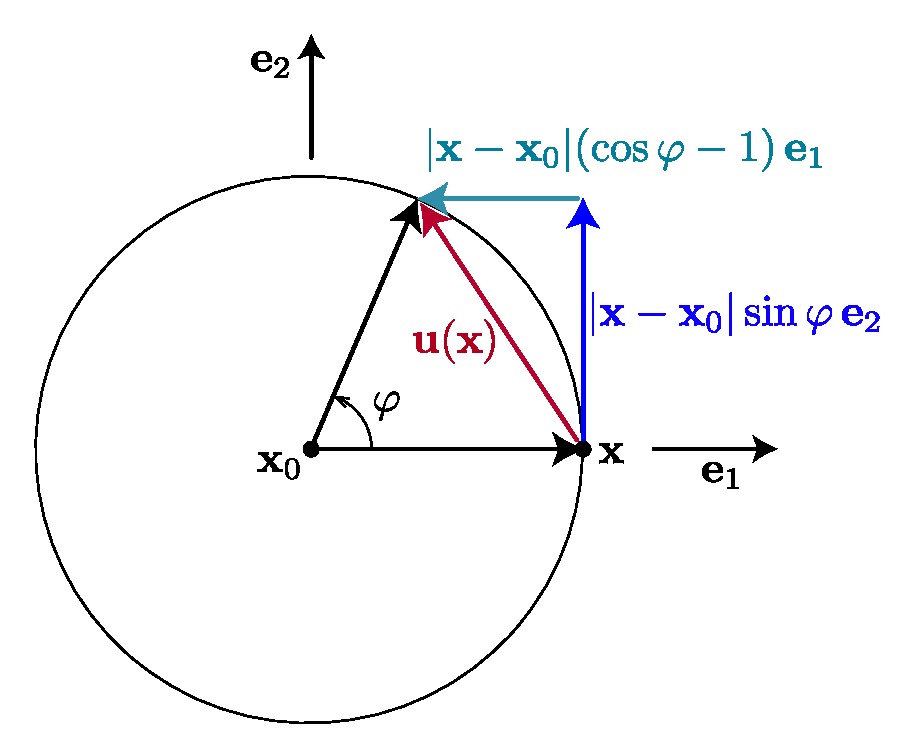
\includegraphics[width=0.5\linewidth]{figure/cinematica/spost_inf}
%	\caption{Rotazione rigida esatta.}
%	\label{fig:spostinf}
%\end{figure}
%
%Ci proponiamo a questo punto di determinare, se possibile, il punto $\xb_C$ del piano cui il corpo appartiene tale che
%\begin{equation}
%	\ub_{\rm rig}(\xb)=\varphi \,\eb_3\times(\xb-\xb_C).
%\end{equation}
%Detto in altri termini, ci proponiamo di individuare un punto del piano rispetto al quale lo spostamento rigido si possa riguardare come puramente rotatorio. Chiameremo questo punto \textit{centro  di rotazione}. La condizione definitoria di $\ub_{\rm rig}(\xb_C)=\mathbf{0}$ consente di individuarne facilmente la posizione; infatti, scelto un punto $\xb_0$, possiamo scrivere 
%\begin{equation}
%	\mathbf{0}=\eb_3\times\ub_{\rm rig}(\xb_C)=\eb_3\times \big( \ub(\xb_0)+\varphi \,\eb_3\times (\xb_C-\xb_0) \big)=\eb_3\times  \ub(\xb_0)-\varphi (\xb_C-\xb_0),
%\end{equation}
%dove si è fatto uso del fatto che
%\begin{equation}
%	\eb_3 \times(\eb_3\times \vb)=-\vb \qquad \vb\in \Vc.
%\end{equation}
%
%Concludiamo allora che il punto $\xb_C$ è
%\begin{definition}
%	\begin{equation}\label{xC}
%		\xb_C=\xb_0+\varphi ^{-1}\, \eb_3\times \ub(\xb_0).
%	\end{equation}
%\end{definition}
%Ne segue che il punto $\xb_C$ si deve trovare sulla perpendicolare per $\xb_0$ al vettore $\ub(\xb_0)$. Risulta quindi agevole individuare una procedura grafica (detta di \textit{Chasles}) per determinare il centro  di rotazione: noti gli spostamenti di due punti, il centro di rotazione deve trovarsi nell'intersezione delle perpendicolari per quei due punti ai rispettivi spostamenti. Se gli spostamenti di due punti sono paralleli, il centro di rotazione si troverà nel punto all'infinito delle rette perpendicolari agli spostamenti e il corpo subirà una traslazione nella direzione comune agli spostamenti dei due punti.
%
%\begin{figure}
%	\centering
%	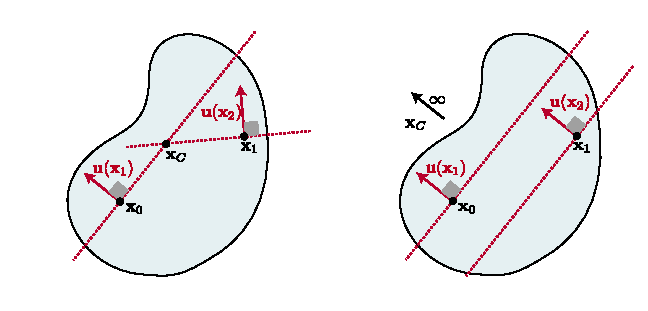
\includegraphics[scale=1.3]{figure/cinematica/chasles}
%	\caption{Costruzione di Chasles per la determinazione del centro  di rotazione.}
%	\label{fig:chasles}
%\end{figure}
%
%
%
%\begin{exercise}
%Si consideri il rettangolo in figura, soggetto ad una rotazione infinitesima antioraria $\varphi$ attorno al punto $A$. Determinare il campo di spostamento e disegnare la configurazione deformata.
%\begin{center}
%	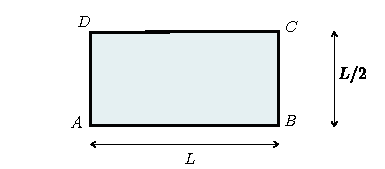
\includegraphics[scale=1.3]{figure/cinematica/rettangolo}
%\end{center}
%\begin{svolgimento}
%Il punto $A$ è il centro di rotazione. Il campo di spostamento assume la forma
%\begin{equation}
%\ub(\xb)=\varphi\eb_3\times \xb.
%\end{equation}
%Per disegnare la configurazione deformata, troviamo lo spostamento dei vertici, scegliendo $A$ come origine:
%\begin{equation}
%\begin{aligned}
%&	\ub(\xb_B)=\varphi\eb_3\times\xb_B=\varphi\eb_3 \times L \eb_1=\varphi L \eb_2,\\
%& \ub (\xb_C)=\varphi\eb_3\times\xb_C=\varphi\eb_3 \times \left( L \eb_1+\frac{L}{2}\eb_2\right)=-\varphi \frac L2 \eb_1+\varphi L\eb_2,\\
%&\ub(\xb_D)=\varphi\eb_3\times\xb_D=\varphi\eb_3 \times L \eb_2=-\varphi L \eb_1.\\
%\end{aligned}
%\end{equation}
%Visto che lo spostamento è una funzione lineare di $\xb$, è facile rappresentare graficamente dei digrammi contenenti le componenti orizzontali e verticali di spostamento, a partire dal punto di nullo rappresentato dal centro di rotazione.
%\begin{center}
%	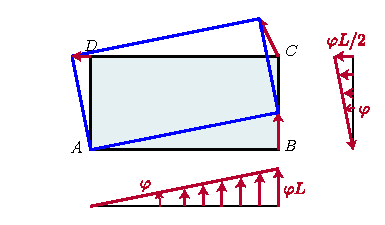
\includegraphics[scale=1.3]{figure/cinematica/rettangolo1}
%\end{center}
%
%\end{svolgimento}
%
%\end{exercise}
%

\subsection{Variazioni geometriche}
\subsubsection{Variazione di lunghezza}
Ricordando la 	\eqref{dl}, il rapporto tra la lunghezza deformata e indeformata di un segmento infinitesimo in direzione $\tb$, trascurando i termini superlineari in $\Hb$, può essere calcolata come
\begin{equation}
\frac{d\ell}{d\ell_0}=|\Fb\tb|=\sqrt{\Cb\tb\cdot\tb}=\sqrt{(\Ib+2\Eb)\tb\cdot\tb}=(\Ib+\Eb)\tb\cdot\tb=1+\Eb\tb\cdot\tb.
\end{equation}
Pertanto, in teoria infinitesima, la variazione specifica di lunghezza in direzione $\tb$ vale
\begin{definition}
	\begin{equation}\label{Ett}
\frac{d\ell-d\ell_0}{d\ell_0}=\frac{d\ell}{d\ell_0}-1=\Eb\tb\cdot\tb.
\end{equation}
\end{definition}

\subsubsection{Variazione di volume}
Senza ledere generalità, consideriamo un volume elementare generato dai vettori della base, in modo che $dv_0=\eb_1\times\eb_2\cdot\eb_3=1$. Il volume deformato sarà allora
\begin{equation}
	\begin{aligned}
	dv&=\Fb\eb_1\times\Fb\eb_2\cdot\Fb\eb_3=\det\mathbf{F}=\det(\Ib+\Hb)=(\Ib+\Hb)\eb_1\times(\Ib+\Hb)\eb_2\cdot(\Ib+\Hb)\eb_3\\
	&=\mathbf{e}_{1}\times\mathbf{e}_{2}\cdot\mathbf{e}_{3}+\mathbf{H}\mathbf{e}_{1}\times\mathbf{e}_{2}\cdot\mathbf{e}_{3}+\mathbf{e}_{1}\times\mathbf{H}\mathbf{e}_{2}\cdot\mathbf{e}_{3}+\mathbf{e}_{1}\times\mathbf{e}_{2}\cdot\mathbf{H}\mathbf{e}_{3}\\&=1+\mathbf{e}_{2}\times\mathbf{e}_{3}\cdot\mathbf{H}\mathbf{e}_{1}+\mathbf{e}_{3}\times\mathbf{e}_{1}\cdot\mathbf{H}\mathbf{e}_{2}+\mathbf{e}_{1}\times\mathbf{e}_{2}\cdot\mathbf{H}\mathbf{e}_{3}\\&=1+\mathbf{H}\mathbf{e}_{1}\cdot\mathbf{e}_{1}+\mathbf{H}\mathbf{e}_{2}\cdot\mathbf{e}_{2}+\mathbf{H}\mathbf{e}_{3}\cdot\mathbf{e}_{3}=1+\operatorname{tr}\mathbf{H}=1+\operatorname{tr}\mathbf{E},
\end{aligned}
\end{equation}
visto che $\operatorname{tr}\Wb=0$. Risulta dunque che, in teoria infinitesima, la variazione di volume vale
\begin{equation}
	\frac{dv}{dv_0}=1+\operatorname{tr}\Eb,
\end{equation}
ovvero
\begin{definition}
	\begin{equation}\label{trE}
	\frac{dv-dv_0}{dv_0}=\operatorname{tr}\mathbf{E}.
\end{equation}
\end{definition}


\subsubsection{Variazione d'area}
Senza ledere generalità, supponiamo di considerare un'area generata dai vettori $\eb_1$ e $\eb_2$, la cui normale referenziale è $\nb_R=\eb_1\times\eb_2=\eb_3$. L'area infinitesima iniziale è $da_0=|\nb_R|=1$. Trascurando i termini superlineari in $\Hb$, l'area deformata vale
\begin{equation}
\begin{aligned}
	da&=|\Fb\eb_1\times\Fb\eb_2|=|(\Ib+\Hb)\eb_1\times(\Ib+\Hb)\eb_2|\\
	&=\sqrt{1+2\eb_3\cdot(\eb_1\times\Hb\eb_2+\Hb\eb_1\times\eb_2)}=\sqrt{1+2(\Hb\eb_1\cdot\eb_1+\Hb\eb_2\cdot\eb_2)}\\
	&=1+E_{11}+E_{22}=1+(\Ib-\eb_3\otimes\eb_3)\cdot\Eb.
\end{aligned}
\end{equation}
Concludiamo allora che, se $\nb_R$ è la normale alla superficie referenziale, allora
\begin{definition}
	\begin{equation}\label{da}
\frac{da-da_0}{da_0}=\frac{da}{da_0}-1=(\Ib-\nb_R\otimes\nb_R)\cdot\Eb,
\end{equation}
\end{definition}
ovvero la variazione specifica d'area è pari alla traccia del tensore di deformazione ristretta al piano in cui si trova l'area considerata.

\subsubsection{Variazione d'angolo}
Consideriamo due vettori ortogonali $\eb_{1}$ e $\eb_2$ passanti per lo stesso punto. L'angolo iniziale è $\alpha_0=\pi/2$, mentre a deformazione avvenuta
\begin{equation}
	\alpha=\arccos\left(\frac{\mathbf{F^{\top}Fe}_1\cdot\mathbf{e}_2}{|\mathbf{F^{\top}Fe}_1\cdot\mathbf{e}_1|^{1/2}|\mathbf{F^{\top}Fe}_2\cdot\mathbf{e}_2|^{1/2}}\right).
\end{equation}
Poiché
\begin{equation}
	\mathbf{F^{\top}Fe}_1\cdot\mathbf{e}_2=(\mathbf{I}+2\mathbf{E})\mathbf{e}_1\cdot\mathbf{e}_2=2\mathbf{Ee}_1\cdot\mathbf{e}_2
\end{equation}
e 
\begin{equation}
	\mathbf{|F^{\top}Fe}_1\cdot \eb_1|^{1/2}=\mathbf{|(I+2E)e}_1\cdot \eb_1|^{1/2}=(1+2\Eb\eb_1\cdot \eb_2)^{1/2}=1+\Eb\eb_1\cdot \eb_1
\end{equation}
si ha che
\begin{equation}
	\begin{aligned}
		\cos\alpha & \Large=\frac{2\mathbf{Ee}_1\cdot\mathbf{e}_2}{(1+\mathbf{Ee}_1\cdot\mathbf{e}_1)(1+\mathbf{Ee}_2\cdot\mathbf{e}_2)}=\frac{2\mathbf{Ee}_1\cdot\mathbf{e}_2}{1+\mathbf{Ee}_1\cdot\eb_1+\mathbf{Ee}_2\cdot\eb_2}  \\
		&=\frac{2\mathbf{Ee}_1\cdot\eb_2}{1+\mathbf{Ee}_1\cdot\eb_1+\mathbf{Ee}_2\cdot\eb_2}\frac{1-\mathbf{Ee}_1\cdot\eb_1-\mathbf{Ee}_2\cdot\eb_2}{1-\mathbf{Ee}_1\cdot\eb_1-\mathbf{Ee}_2\cdot\eb_2} \\
		&=2\mathbf{Ee}_1\cdot\eb_2(1-\mathbf{Ee}_1\cdot\eb_1-\mathbf{Ee}_2\cdot\eb_2) \\
		&=2\mathbf{Ee}_1\cdot\eb_2.
	\end{aligned}
\end{equation}
Calcoliamo dunque la variazione d'angolo
\begin{equation}
	\delta\alpha=\alpha-\alpha_0=\alpha-\frac{\pi}{2}.
\end{equation}
Poiché
\begin{equation}
	\sin(\delta\alpha)=\sin(\frac\pi2-\alpha)=\cos\alpha,
\end{equation}
si ricava che
\begin{equation}
	\begin{aligned}\delta\alpha&=\arcsin(\cos\alpha)=\arcsin(2\mathbf{Ee}_1\cdot\mathbf{e}_2)=2\mathbf{Ee}_1\cdot\mathbf{e}_2,\end{aligned}
\end{equation}
che si ottiene  utilizzando l’espansione in serie di Taylor dell'arcoseno: $\arcsin x=x+o(x)$ per $x\to 0$ e quindi
\begin{definition}
	\begin{equation}\label{E12}
	\begin{aligned}\delta\alpha=2\mathbf{Ee}_1\cdot\mathbf{e}_2,\end{aligned}
\end{equation}
\end{definition}


\subsection{Componenti del tensore della deformazione infinitesima}
Scelta una base cartesiana $\{\eb_i\}$, del tensore della deformazione infinitesima si può dare la seguente rappresentazione matriciale:
\begin{equation}
	[\Eb]=\begin{bmatrix}E_{11}&E_{12}&E_{13}\\E_{21}&E_{22}&E_{23}\\E_{31}&E_{32}&E_{33}\end{bmatrix}=\begin{bmatrix}E_{11}&E_{12}&E_{13}\\&E_{22}&E_{23}\\\mathrm{sym}&&E_{33}\end{bmatrix}.
\end{equation}

L'interpretazione di $E_{11}$ è immediata, ricordando la \eqref{Ett}:
\begin{equation}
	E_{11}=\Eb\eb_1\cdot\eb_1=\frac{d\ell-d\ell_0}{d\ell_0},
\end{equation}
ovvero rappresenta l'allungamento specifico  lungo la direzione $\eb_1$. Analoga interpretazione può darsi per tutte le componenti sulla diagonale.

Per interpretare $E_{12}$, occorre ricorrere alla  \eqref{E12}: 
\begin{equation}
E_{12}=\Eb\eb_1\cdot\eb_2=\frac{\delta\alpha}{2},
\end{equation}
ovvero rappresenta la metà dell’angolo di scorrimento lungo le direzioni $\eb_1$ ed $\eb_2$. Analoga interpretazione è possibile fornire per $E_{13}$ e $E_{23}$. 

Osserviamo inoltre che $\operatorname{tr}\Eb=E_{11}+E_{22}+E_{33}$, vista la \eqref{trE}, rappresenta la variazione specifica di un volume infinitesimo generato dai tre vettori della base. Infine, alla luce della \eqref{da}, la somma $E_{11}+E_{22}$ rappresenta la variazione specifica d'area nel piano generato da $\eb_{1}$ e $\eb_2$; analoga interpretazione si dà della somma di qualunque coppia di elementi della diagonale principale.

\subsection{Deformazioni elementari}
In questa sezione analizziamo alcune deformazioni omogenee significative.

\subsubsection{Estensione uniforme}
In un'estensione uniforme di $\varepsilon$ in direzione $\nb$ ($|\nb|=1$), il campo di spostamento è dato da
\begin{equation}
	\mathbf{u}(\mathbf{x})=\varepsilon\,\mathbf{n}\otimes\mathbf{n}(\mathbf{x}-\mathbf{x}_{0}).
\end{equation}
Il generico punto $\xb$ si sposta dunque in direzione $\nb$, in maniera linearmente crescente man mano che $\xb$ si allontana dal punto fisso $\xb_0$.


\begin{center}
		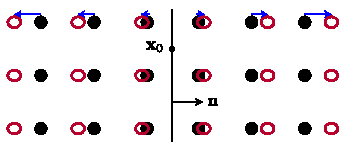
\includegraphics[scale=1.3]{figure/cinematica/estensione}
\end{center}


 In questo caso
\begin{equation}
\nabla\ub=\varepsilon\,\nb\otimes\nb=\Eb.
\end{equation}
Poiché 
\begin{equation}
	\varepsilon=\Eb\nb\cdot\nb
\end{equation}
la costante $\varepsilon$ rappresenta l'allungamento specifico in direzione $\nb$. 

Se $\mb$ è un vettore ortogonale a $\nb$, poiché $\Eb\nb \cdot\mb=0$, l'angolo tra una fibra diretta come $\nb$ ed una come $\mb$ non varia. Inoltre, dato che $\Eb\mb \cdot\mb=0$, nella direzione $\mb$ non c'è alcuna variazione di lunghezza.

\subsubsection{Dilatazione uniforme}
In una dilatazione di $\kappa$ attorno a $\xb_0$ il campo di spostamento è
\begin{equation}
\ub(\xb)=\kappa(\xb-\xb_0).
\end{equation}
Tutti i punti si spostano dunque nella direzione radiale $\xb -\xb_0$, di una quantità linearmente crescente man mano che ci si allontana da $\xb_0$.

\begin{center}
	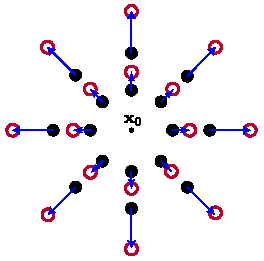
\includegraphics[scale=1.3]{figure/cinematica/dilatazione}
\end{center}

In questo caso
\begin{equation}
\nabla\ub=\kappa \Ib=\Eb.
\end{equation}
Una fibra in direzione $\tb$ qualunque presenta un allungamento specifico
\begin{equation}
\Eb\tb\cdot\tb=\kappa.
\end{equation}
La variazione specifica di volume è
\begin{equation}
\frac{dv-dv_0}{dv}=\operatorname{tr}\Eb=3\kappa.
\end{equation}

\subsubsection{Scorrimento}
Si consideri un punto $\xb_0$ e due vettori unitari $\nb$ e $\mb$ mutuamente ortogonali. In uno scorrimento lungo $\nb$ e $\mb$ lo spostamento di un punto $\xb$ è diretto come $\mb$ e il suo modulo è proporzionale alla distanza tra $\xb$ e il piano di normale $\nb$ passante per $\xb_0$:
\begin{equation}
\ub(\xb)=\gamma\big( (\xb-\xb_0)\cdot\nb \big)\mb=\gamma \mb\otimes\nb (\xb -\xb_0).
\end{equation}

\begin{center}
	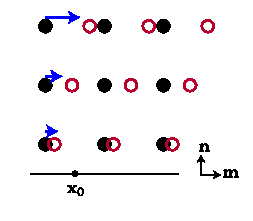
\includegraphics[scale=1.3]{figure/cinematica/scorrimento}
\end{center}

Poiché $\nabla\ub=\gamma \mb \otimes \nb$, deduciamo che
\begin{equation}
\Eb=\frac{\gamma}{2}(\mb \otimes \nb +\nb \otimes \mb), \qquad \Wb=\frac{\gamma}{2}(\mb \otimes \nb-\mb \otimes \nb).
\end{equation}
Facendo ricorso alla \eqref{E12}, deduciamo immediatamente che
\begin{equation}
	\frac{\delta\alpha}{2}=\Eb \mb \cdot\nb=\frac{\gamma}{2},
\end{equation}
e quindi il coefficiente di scorrimento $\gamma$ è pari alla variazione d'angolo tra $\mb$ e $\nb$. Fissiamo per comodità $\xb_0=\mathbf{0}$, $\mb =\eb_1$ e $\nb=\eb_2$. Allora, le matrici rappresentative di $\Eb$ e $\Wb$ risultano:
\begin{equation}
	[\mathbf{E}(\mathbf{u})]=\frac{\gamma}{2}\begin{bmatrix}0&1&0\\1&0&0\\0&0&0\end{bmatrix}\quad\mathrm{e}\quad[\mathbf{W}(\mathbf{u})]=\frac{\gamma}{2}\begin{bmatrix}0&1&0\\-1&0&0\\0&0&0\end{bmatrix}.
\end{equation}
Dato che $\ub (\xb)=\Eb \xb +\Wb \xb$, concludiamo che
\begin{equation}
\ub(\xb)=\underbrace{\frac{\gamma}{2}(x_2 \eb_1+x_1 \eb_2)}_{\text{scorrimento puro}} +\underbrace{ \frac{\gamma}{2}(x_2 \eb_1-x_1 \eb_2)}_{\text{rotazione infinitesima}}.
\end{equation}
e dunque lo spostamento complessivo può essere visto come la somma di uno scorrimento puro (dato da $\Eb \xb$) e una rotazione infinitesima (data da $\Wb \xb$).  

\begin{center}
	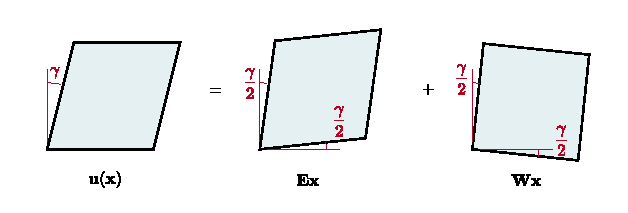
\includegraphics[scale=1.3]{figure/cinematica/scorrimento1}
\end{center}

Alla luce dell'osservazione \ref{skvec}, l'assiale di $\Wb$ è
\begin{equation}
\wb =-\frac{\gamma}{2}\, \eb_3.
\end{equation}
Si tratta dunque di una rotazione attorno all'asse $\eb_3$, di angolo $\gamma/2$; il segno negativo indica che la rotazione è oraria.

\begin{exercise}
Dato il campo di spostamenti
\begin{equation}
	\ub(\xb)=(\alpha_1 x_1x_2+\alpha_2 x_2)\eb_1+(\beta_1 x_2+\beta_2 x_1)\eb_2, \qquad \alpha_1, \alpha_2, \beta_1, \beta_2\in \Ro,
\end{equation}
 determinare:
\begin{enumerate}
	\item Il contorno deformato di un quadrato di lato $L$ con due lati sugli assi $x_1, x_2$;
	\item 	il tensore di deformazione infinitesima e  il tensore di rotazione infinitesima;
	\item la configurazione finale e la variazione di lunghezza (utilizzando la teoria infinitesima) della diagonale inclinata di $\pi/4$ rispetto a $x_1$;
	\item la variazione di area (utilizzando la teoria infinitesima) del quadrato
	introdotto nel punto a).
\end{enumerate}

\begin{svolgimento}
	\begin{enumerate}
		\item Con riferimento alla notazione in figura,
		\begin{center}
			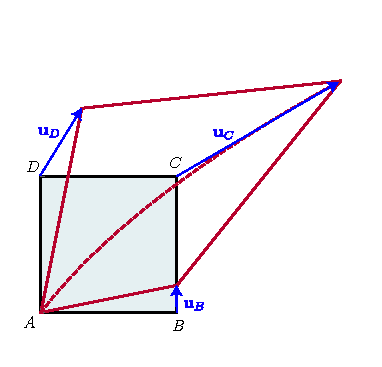
\includegraphics[scale=1]{figure/cinematica/esempio3d_1}
		\end{center}
		possiamo immediatamente calcolare lo spostamento dei vertici:
		\begin{equation}
			\ub_A=\mathbf{0}, \qquad \ub_B=\beta_2 L \eb_2, \qquad \ub_C=(\alpha_1^2L+\alpha_2L)\eb_1+(\beta_1+\beta_2)L\eb_2, \qquad \ub_D=\alpha_2L \eb_1+\beta_1 L \eb_2.
		\end{equation}
		I punti del lato  $AB=\{ \xb\in \Vc \,:\, \xb =x_1\eb_1, 0<x_1<L\}$ subiscono la deformazione
		\begin{equation}
			\fb(\xb)=x_1\eb_1+(x_2+\beta_2 x_1)\eb_2,
		\end{equation}
		e dunque il lato rimane rettilineo. Per disegnarne la deformata è sufficiente unire i vertici. È facile verificare che anche tutti gli altri lati restano rettilinei, sicché il bordo della regione deformata è ottenibile semplicemente unendo i vertici.
	\item Calcoliamo il gradiente dello spostamento:
	\begin{equation}
	\Hb=\ub,_i\otimes\eb_i=\alpha_1x_2 \eb_1\otimes \eb_1+\beta_2\eb_2\otimes\eb_1+(\alpha_1x_1+\alpha_2)\eb_1\otimes\eb_2+\beta_1\eb_2\otimes\eb_2,
	\end{equation}
	da cui
	\begin{equation}
	\Eb=\alpha_1x_2 \eb_1\otimes \eb_1+\frac12 (\alpha_1x_1+\alpha_2+\beta_2)(\eb_1\otimes\eb_2+\eb_2\otimes \eb_1)+\beta_1\eb_2\otimes\eb_2,
	\end{equation}
	e
	\begin{equation}
	\Wb=\frac12 (\alpha_1 x_1+\alpha_2-\beta_2)(\eb_1\otimes\eb_2-\eb_2\otimes\eb_1).
	\end{equation}
Osserviamo che l'assiale di $\Wb$ è il vettore $-\frac12 (\alpha_1 x_1+\alpha_2-\beta_2)\eb_3$ e dunque i punti subiscono un rotazione attorno ad $\eb_3$ dell'angolo specificato da $-\frac12 (\alpha_1 x_1+\alpha_2-\beta_2)$.
\item La diagonale è l'insieme $\{\xb_d\in \Vc\,:\, \xb_d=x_1(\eb_1+\eb_2), 0<x_1<L\}$, che dunque viene trasformato nell'insieme
\begin{equation}
	\fb(\xb_d)=\ub(\xb_d)+\xb_d=(\alpha_{1}x_{1}^{2}+\alpha_{2}x_{1}+\alpha_{1})\eb_{1}+(1+\beta_{1}+\beta_{2})x_{1}\eb_{2},
\end{equation}
che è l'equazione parametrica di una curva nel piano.
	\end{enumerate}
	Definendo
	\begin{equation}
		\tb=\frac{\overrightarrow{AC}}{|\overrightarrow{AC}|}=\frac{\eb_{1}+\eb_{2}}{\sqrt{2}}
	\end{equation}
	il versore della diagonale, determiniamo l'allungamento specifico in teoria infinitesima
	\begin{equation}
		\Eb(\xb_{d})\tb\cdot\tb=\frac{1}{2}(2x_{1}\alpha_{1}+\alpha_{2}+\beta_{1}+\beta_{2})=\frac{d\ell}{d\ell_0}-1,
	\end{equation}
dove $d\ell_0=\sqrt2 \dd x_1$, 
da cui la lunghezza finale della diagonale
\begin{equation}
\begin{aligned}
	d\ell=	\sqrt{2}\big(1+\Eb(\xb_{d})\tb\cdot\tb\big)\dd x_1\quad \Longrightarrow   \quad \ell&=\sqrt{2}L+\sqrt{2}\int_0^L\frac{1}{2}(2x_{1}\alpha_{1}+\alpha_{2}+\beta_{1}+\beta_{2})\dd x_1\\
	&=\sqrt{2}L+\frac{\sqrt{2}L}{2}(\alpha_1 L+\alpha_2+\beta_1+\beta_2).
\end{aligned}
\end{equation}
\item La variazione specifica d'area in teoria infinitesima è
\begin{equation}
	\frac{d a}{da_0}=1+\operatorname{tr}\Eb=1+\alpha_1 x_1+\beta_1,
\end{equation}
da cui
\begin{equation}
a=\int_0^L\int_0^L(1+\alpha_1 x_1+\beta_1)\dd x_1\dd x_2=\frac{L^2}{2}(2+\alpha_1 L+2\beta_1).
\end{equation}
\end{svolgimento}

\end{exercise}

\begin{exercise}
Una \textit{rosetta estensimetrica} è un dispositivo elettromeccanico che misura l'allungamento percentuale in tre direzioni. Montando un tale dispositivo sulla superficie di una struttura, è possibile determinare le deformazioni assiali in certe direzioni. Una rappresentazione schematica di una rosetta è rappresentata in  figura. Si assuma che in un esperimento si siano misurate gli allungamenti specifici nelle direzioni individuate dai versori $\ab$, $\bb$ e $\cb$ e che sia risultato $\varepsilon_a$, $\varepsilon_b$ e $\varepsilon_c$. Usando la teoria infinitesima, si determinino le componenti di allungamento specifico nelle direzioni $\eb_1$ e $\eb_2$ e la variazione d'angolo $\eb_1$ e $\eb_2$.
%
\begin{center}
		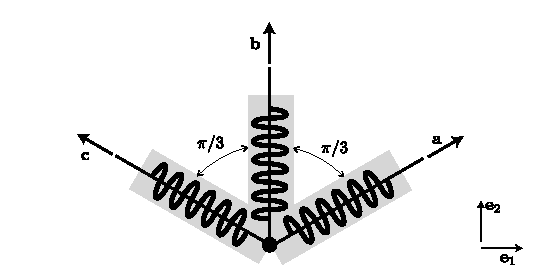
\includegraphics[scale=1.2]{figure/cinematica/rosetta.pdf}
\end{center}

\begin{svolgimento}
Indichiamo con
\begin{equation}
\ab = \frac{\sqrt{3}}{2}\eb_{1}+\frac12 \eb_2, \qquad \bb=\eb_2, \qquad \cb=-\frac{\sqrt{3}}{2}\eb_{1}+\frac12 \eb_2
\end{equation}
i versori che individuano le tre direzioni della rosetta. Occorre risolvere il sistema
\begin{equation}
\begin{cases}
\Eb \ab \cdot \ab=\dfrac{1}{2}(3 E_{11}+2\sqrt{3} E_{12}+E_{22})=\varepsilon_a,\\[.2cm]
\Eb \bb \cdot\bb=E_{22}=\varepsilon_b,\\[.2cm]
\Eb \cb \cdot\cb_1=\dfrac14 (3E_{11}-2\sqrt{3}E_{12}+E_{22})=\varepsilon_c,
\end{cases}
\end{equation}
nelle tre incognite $E_{11}$, $E_{12}$, $E_{22}$. La soluzione è
\begin{equation}
E_{11}=\frac13(2\varepsilon_a-\varepsilon_b+2\varepsilon_c), \qquad E_{12}=\frac{\varepsilon_a-\varepsilon_c}{\sqrt{3}}, \qquad 
E_{22}=\varepsilon_b.
\end{equation}
\end{svolgimento}

\end{exercise}

\begin{exercise}\label{defmedia}
Sia $\bar\Eb$ la deformazione media di una configurazione ${\Omega}$:
\begin{equation}
	\bar{\Eb}=\frac{1}{\textrm{vol}({\Omega})}\int_{\Omega}\Eb.
\end{equation}
Dimostrare che la deformazione media dipende soltanto dallo spostamento $\ub$ sulla frontiera e, in particolare,
\begin{equation}
	\bar{\Eb}=\frac{1}{2\textrm{vol}(\Omega)}\int_{\partial{\Omega}}\ub\otimes\nb+\nb\otimes\ub
\end{equation}
dove $\textrm{vol}(\Omega)$ è il volume di $\Omega$  e $\nb$ la normale alla frontiera di ${\Omega}$. 

\begin{svolgimento}
Utilizziamo la seguente versione del teorema dalla divergenza (v. \eqref{theodiv}):
\begin{equation}
\int_{\Omega}\nabla \varphi=\int_{\partial\Omega}\varphi\nb,
\end{equation}
dove $\varphi$ è un campo scalare. Scegliamo $\varphi=\ub \cdot\ab$, con $\ab\in\Vc$ costante. Si ha
\begin{equation}
(\nabla \varphi)_i=\varphi,_i \eb_i=(\ub,_{i}\cdot \ab)\eb_i=(\eb_i \otimes \ub,_i)\ab=\nabla\ub ^\top \, \ab.
\end{equation}
Pertanto
\begin{equation}
\left( \int_{\Omega}\nabla\ub ^\top  \right)\ab =\int_{\partial{\Omega}}(\ub\cdot\ab)\nb=\int_{\partial{\Omega}}(\nb \otimes \ub)\ab,
\end{equation}
da cui concludiamo che 
\begin{equation}
\int_{\Omega}\nabla\ub ^\top =\int_{\partial{\Omega}}\nb \otimes \ub.
\end{equation}
Data la definizione di $\Eb$, è allora immediato concludere che
\begin{equation}
	\bar{\Eb}=\frac{1}{2\operatorname{vol}(\Omega)}\int_{\partial{\Omega}}\ub\otimes\nb+\nb\otimes\ub.
\end{equation}
\end{svolgimento}
\end{exercise}

\begin{exercise}
	\item Si consideri un disco di raggio $R$ centrato nell'origine del sistema di riferimento cartesiano $\{O; x_1, x_2\}$. Sulla frontiera del disco è imposto uno spostamento
	\begin{equation}
		\ub(\xb)=(\alpha\eb_1\otimes\eb_1+\beta\eb_2\otimes\eb_1)\xb \qquad \alpha,\beta\in\Ro.
	\end{equation}
	Determinare la deformazione media del disco.
\begin{svolgimento}
Vista la geometria, conviene usare un sistema di coordinate polari, in modo che la posizione del generico punto del disco sia
\begin{equation}
\xb=\rho \cos\vartheta \eb_1+ \rho \sin \vartheta\eb_2, \qquad 0\leq\rho<R, \quad 0\leq \vartheta<2\pi.
\end{equation}
Il vettore unitario normale al disco è 
\begin{equation}
	\nb= \cos\vartheta \eb_1+  \sin \vartheta\eb_2.
\end{equation}
Con l'obiettivo di utilizzare il risultato dell'esercizio \ref{defmedia}
determiniamo
\begin{equation}
\begin{aligned}
	\frac12	(\ub\otimes\nb+\nb\otimes\ub)&=\alpha R \cos^2 \vartheta \eb_1\otimes \eb_1+\frac{1}{2} R \cos\vartheta(\alpha\sin\vartheta+\beta\cos\vartheta)(\eb_1\otimes\eb_2+\eb_2\otimes \eb_1)\\
	&+R \beta \sin\vartheta\cos\vartheta\,\eb_2\otimes\eb_2,
\end{aligned}
\end{equation}
 da cui
 \begin{equation}
 	\bar{\Eb}=\frac{1}{\pi R^2}\int_0^{2\pi}\frac12	(\ub\otimes\nb+\nb\otimes\ub)R \dd \vartheta=\alpha \eb_1\otimes\eb_1+\frac \beta2(\eb_1\otimes\eb_2+\eb_2\otimes \eb_1).
 \end{equation}
\end{svolgimento}
\end{exercise}

\begin{exercise}
	Sia  $\ub\;:\;\Omega\to\Vc$  un campo di spostamento tangente alla frontiera di $\Omega$. Mostrare che in teoria infinitesima la variazione specifica di volume è in media nulla.
	\begin{svolgimento}
Utilizzando il risultato dell'esercizio \ref{defmedia}, possiamo determinare la media della  variazione specifica di volume:
\begin{equation}
\operatorname{tr}\bar{\Eb}=\frac{1}{\operatorname{vol}(\Omega)}\int_{\partial{\Omega}}\ub \cdot \nb=0
\end{equation}
visto che $\ub \cdot \nb=0$ su $\partial{\Omega}$, essendo $\ub$ tangente alla frontiera di $\Omega$.
	\end{svolgimento}
\end{exercise}

\subsection{La condizione di compatibilità}
Dato un arbitrario campo di deformazione $\Eb$, la relazione tra spostamento e deformazione
\begin{equation}
	\Eb=\frac12(\nabla\ub +\nabla\ub^\top)
\end{equation}
costituisce un'equazione differenziale  lineare del primo ordine nel campo di spostamento $\ub$, la cui soluzione non è garantita esistere. Mostreremo che una condizione \textit{necessaria} per l'esistenza di soluzioni è che il campo di deformazione soddisfi una certa condizione di compatibilità, che è anche \textit{sufficiente} a garantire l'esistenza se il dominio è semplicemente connesso.

Per prima cosa osserviamo che il campo di deformazione $\Eb$ e il vettore della rotazione infinitesima $\wb$ soddisfano la seguente condizione:
\begin{equation}\label{RotE}
	\Rot \Eb=\nabla \wb.
\end{equation}
%Ricordiamo che le componenti del rotore di un vettore $\vb$ sono 
%\begin{equation}
%(\Rot \vb)_i=	\epsilon_{ijk}v_{k,j}
%\end{equation}
%dove
%\begin{equation}
%\epsilon_{ijk}=\eb_i\times\eb_j\cdot\eb_k
%\end{equation}
%è il simbolo di Ricci (v. \eqref{Ricci}).
%, tale che 
%\begin{equation}\epsilon_{ijk}=\begin{cases}+1&\text{se tutti gli indici $i,j,k$ sono diversi e la loro sequenza}\\&\text{ è una permutazione di classe pari di $1,2,3$};\\0&\text{se almeno due degli indici $i, j, k$ sono uguali;}\\-1&\text{se tutti gli indici  $i,j,k$ sono diversi e la loro sequenza}\\&\text{è una permutazione di classe dispari di $1,2,3$}\end{cases}
%\end{equation}
%Dato un campo tensoriale $\Ab$ il suo rotore è così definito:
%\begin{equation}
%(\Rot \Ab)\ab \coloneqq \Rot(\Ab^\top \ab), \qquad \forall \ab \in \Vc;
%\end{equation}
%in componenti:
%\begin{equation}
%	(\Rot\Ab)_{ij}=\epsilon_{ipq}A_{jq},_{p}.
%\end{equation}
Per dimostrare la \eqref{RotE}, calcoliamo il rotore del gradiente dello spostamento (v. \eqref{RotT}):
\begin{equation}
	(\Rot(\nabla\ub))_{ij}=\epsilon_{ipq}(\nabla\ub)_{jq,p}=\epsilon_{ipq}(u_{j,q}),p=\epsilon_{ipq}u_{j,qp}=0;
\end{equation}
inoltre si ha che 
\begin{equation}
	(\Rot(\nabla\ub^\top))_{ij}=\epsilon_{ipq}(u_{q,j}),_p=\epsilon_{ipq}u_{q,jp}=(\epsilon_{ipq}u_{q,p}),_j=2 w_{i,j}=2 (\nabla \wb)_{ij}.
\end{equation}
Nell'ultima uguaglianza si è introdotto il vettore
\begin{equation}
	\wb \coloneqq \frac12 \Rot \ub;
\end{equation}
poiché, facendo uso della \eqref{epsdel}, possiamo scrivere la seguente successione di eguaglianze,
\begin{equation}
	\begin{aligned}
(\wb \times \ab)_i &=\epsilon_{ijk}w_j a_k=\frac12\epsilon_{ijk}\epsilon_{jpq}u_{q,p}a_k=-\frac12\epsilon_{jik}\epsilon_{jpq}u_{q,p}a_k=-\frac{1}{2}(\delta_{ip}\delta_{kq}-\delta_{iq}\delta_{kp})u_{q,p}a_k\\
&=\frac12 (u_{i,k}-u_{k,i})a_k=\frac{1}{2}(\nabla \ub-\nabla \ub^\top)_{ik}a_k=W_{ik}a_k=(\Wb \ab)_i,
\end{aligned}
\end{equation}
per ogni $\ab$, possiamo identificare $\wb$ con l'assiale del tensore della rotazione infinitesima $\Wb$, sicché
\begin{equation}
	\Wb \ab=\frac{1}{2}\Rot \ub \times \ab.
\end{equation}


Concludiamo allora che 
\begin{equation}
	\Rot \Eb =\frac12\big( \Rot (\nabla \ub) + \Rot (\nabla \ub^\top)=\nabla \wb.
\end{equation}
Applicando nuovamente l'operatore di rotore alla \eqref{RotE}, arriviamo alla conclusione che una condizione necessaria per l'esistenza di un campo di spostamento è che $\Eb$ soddisfi la seguente \textit{condizione di compatibilità}:
\begin{definition}
	\begin{equation}\label{RotRot}
\Rot \Rot \Eb =\mathbf{0}.
\end{equation}
\end{definition}


Dimostriamo adesso che la condizione \eqref{RotRot}, non è solo sufficiente, ma anche necessaria, se il dominio è semplicemente connesso; in altre parole, se $\Rot \Rot \Eb=\mathbf{0}$, allora certamente esiste un campo vettoriale $\ub$ tale che $\Eb =\sym \nabla \ub$.

Per dimostrarlo ci servono due risultati  preparatori:
\begin{enumerate}
	\item Sia $\Tb\in \Lin$ tale che $\Rot \Tb =\mathbf{0}$, allora esiste un campo vettoriale $\ub$ tale che\footnote{Per dimostrarlo, consideriamo i vettori
		\begin{equation}
			\ab_i =\Tb^\top \eb_i,
		\end{equation}
		dove $\eb_i$ sono i vettori della base; si ha che
		\begin{equation}
			\Rot \ab_i= \Rot (\Tb^\top \eb_i)=\Rot(\Tb^\top)\eb_i=0
		\end{equation}
		e dunque esistono dei campi scalari $u_i$ tali che $\ab_i=\nabla u_i$.
		%
		Definiamo $\ub \coloneqq u_i \eb_i$; allora
		\begin{equation}
			\ab_i=\nabla u_i =\nabla(\ub \cdot \eb_i)=(\nabla \ub)^\top\eb_i=\Tb ^\top \eb_i,
		\end{equation}
		da cui deduciamo \eqref{Tnabu}.}
	\begin{equation}\label{Tnabu}
	\Tb=\nabla \ub.
	\end{equation}
\item Sia $\Tb \in \Lin$ tale che $\Rot \Tb=\mathbf{0}$ e $\operatorname{tr}\Tb=0$, allora esiste $\Wb \in \Skw$ tale che\footnote{
Dimostriamolo: sia $\ub$ il vettore definito nella nota precedente e $\Wb$ il tensore antisimmetrico associato a $-\ub$. Allora
\begin{equation}
	\Div \ub = \operatorname{tr}\nabla \ub =\operatorname{tr}\Tb =0.
\end{equation}
In  virtù della \eqref{identitadiff}$_9$
\begin{equation}
	-\Rot \Wb =(\Div \ub)\Ib-\nabla \ub=-\nabla \ub =-\Tb,
\end{equation}
da cui il risultato.
}
\begin{equation}
\Tb=\Rot \Wb.
\end{equation}
\end{enumerate}

Torniamo dunque alla dimostrazione che, se $\Rot \Rot \Eb=\mathbf{0}$, allora  esiste un campo vettoriale $\ub$ tale che $\Eb =\sym \nabla \ub$. Assumiamo che $\Rot\Rot\Eb=\mathbf{0}$ in $\Omega$.  Sia $\Ab =\Rot \Eb$; poiché $\Eb \in \Sym$, 
\eqref{identitadiff}$_8$ implica che
\begin{equation}
\operatorname{tr}\Ab=0.
\end{equation}
Poiché $\Rot \Ab=\mathbf{0}$, allora esiste un campo tensoriale $\Wb\in\Skw$ tale che
\begin{equation}
	\Ab =-\Rot \Wb.
\end{equation}
Visto che $\Ab =\Rot \Eb$,
\begin{equation}
\Rot (\Eb+ \Wb)=\mathbf{0};
\end{equation}
esiste allora un campo vettoriale $\ub$ tale che
\begin{equation}
	\Eb+ \Wb= \nabla \ub.
\end{equation}
Prendendo la parte simmetrica dell'ultima uguaglianza, concludiamo allora che esiste $\ub$ tale che
\begin{equation}
\Eb = \sym \nabla \ub.
\end{equation}









